\documentclass[a4paper]{article}

\usepackage[utf8]{inputenc}
\usepackage[DIV=9]{typearea}
\usepackage{microtype}
\usepackage{mathtools, amssymb}
\usepackage{parskip}
\usepackage{graphicx}
\usepackage{subcaption}
\graphicspath{ {./results} }
\usepackage{float}
\usepackage[colorlinks=true]{hyperref}
\hypersetup{linktoc=all}

\title{3}
\date{}

\begin{document}
\maketitle
\section{Ground Truth Images}
Figure \ref{fig:gt} displays the ground truth images.
\begin{figure}[H]
    \centering
    \begin{subfigure}{0.24\linewidth}
        \centering
        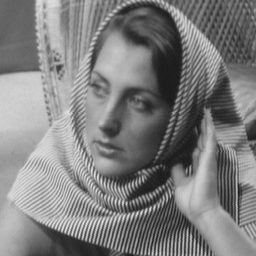
\includegraphics[width = \linewidth]{barbara256.png}
        \caption{Barbara}
    \end{subfigure}
    \begin{subfigure}{0.24\linewidth}
        \centering
        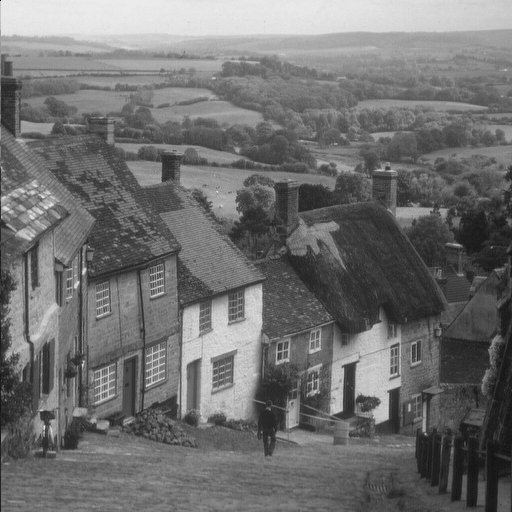
\includegraphics[width = \linewidth]{goldhill.png}
        \caption{Goldhill}
    \end{subfigure}
    \caption{Ground Truth Image}
    \label{fig:gt}
\end{figure}
\section{Noisy Images}
Figure \ref{fig:n} displays the noisy images with noise $\sim\mathcal{N}(0,4)$ with calculated RMSE.
\begin{figure}[H]
    \centering
    \begin{subfigure}{0.24\linewidth}
        \centering
        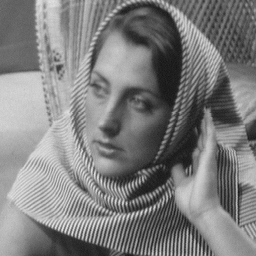
\includegraphics[width = \linewidth]{barbara256 with noise.png}
        \caption{RMSE = 0.014633}
    \end{subfigure}
    \begin{subfigure}{0.24\linewidth}
        \centering
        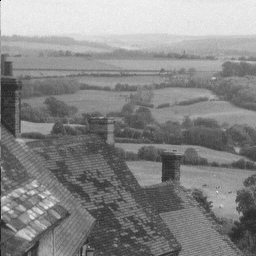
\includegraphics[width = \linewidth]{goldhill with noise.png}
        \caption{RMSE = 0.013943}
    \end{subfigure}
    \caption{Noisy Image}
    \label{fig:n}
\end{figure}
\section{Reconstructed images using ISTA}
As a general observation, noisy and noiseless RMSE in any reconstruction are very close, suggesting that given noise doesn't make a significant difference.
\subsection{All measurements}
\ref{fig:dcta}, \ref{fig:hwa} shows the reconstruction images with all measurements for noisy as well as noiseless images with calculated RMSE. All RMSE values are less than 0.003.
\begin{figure}[H]
    \centering
    \begin{subfigure}{0.24\linewidth}
        \centering
        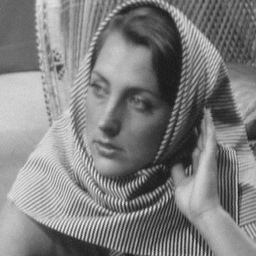
\includegraphics[width = \linewidth]{dct2D/barbara256 reconstructed using all measurements, with noise.png}
        \caption{Noisy, 0.0026952}
    \end{subfigure}
    \begin{subfigure}{0.24\linewidth}
        \centering
        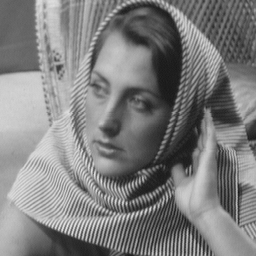
\includegraphics[width = \linewidth]{dct2D/barbara256 reconstructed using all measurements, without noise.png}
        \caption{Noiseless, 0.0026166}
    \end{subfigure}
    \begin{subfigure}{0.24\linewidth}
        \centering
        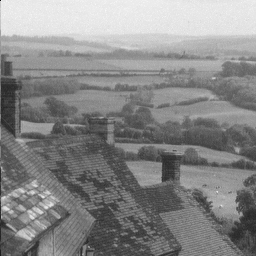
\includegraphics[width = \linewidth]{dct2D/goldhill reconstructed using all measurements, with noise.png}
        \caption{Noisy, 0.0027094}
    \end{subfigure}
    \begin{subfigure}{0.24\linewidth}
        \centering
        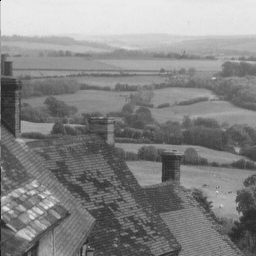
\includegraphics[width = \linewidth]{dct2D/goldhill reconstructed using all measurements, without noise.png}
        \caption{Noiseless, 0.002681}
    \end{subfigure}
    \caption{DCT Basis}
    \label{fig:dcta}
\end{figure}
\begin{figure}[H]
    \centering
    \begin{subfigure}{0.24\linewidth}
        \centering
        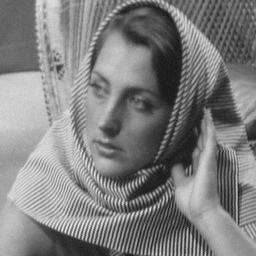
\includegraphics[width = \linewidth]{haarWavelet/barbara256 reconstructed using all measurements, with noise.png}
        \caption{Noisy, 0.0028379}
    \end{subfigure}
    \begin{subfigure}{0.24\linewidth}
        \centering
        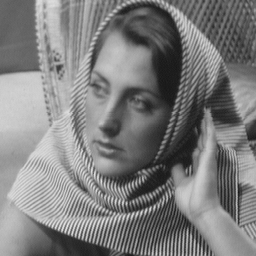
\includegraphics[width = \linewidth]{haarWavelet/barbara256 reconstructed using all measurements, without noise.png}
        \caption{Noiseless, 0.0028216}
    \end{subfigure}
    \begin{subfigure}{0.24\linewidth}
        \centering
        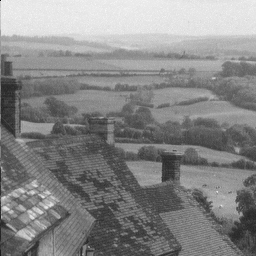
\includegraphics[width = \linewidth]{haarWavelet/goldhill reconstructed using all measurements, with noise.png}
        \caption{Noisy, 0.0028422}
    \end{subfigure}
    \begin{subfigure}{0.24\linewidth}
        \centering
        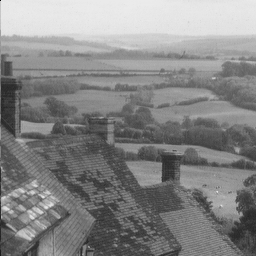
\includegraphics[width = \linewidth]{haarWavelet/goldhill reconstructed using all measurements, without noise.png}
        \caption{Noiseless, 0.0028246}
    \end{subfigure}
    \caption{Haar Wavelet Basis}
    \label{fig:hwa}
\end{figure}
\clearpage
\subsection{Compressive measurements}
\ref{fig:dctb}, \ref{fig:hwb} shows the reconstruction images with compressive measurements for noisy as well as noiseless images using patching with calculated RMSE. This time, all RMSE values are close to 0.54 as they are less bright which could be improved by choosing a suitable value of $\lambda$. Also, the images show weird artifacts around the border which could possibly be improved by padding the image.
\begin{figure}[H]
    \centering
    \begin{subfigure}{0.24\linewidth}
        \centering
        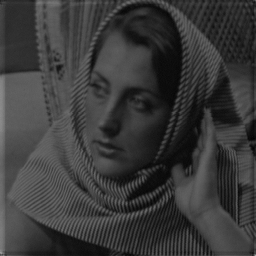
\includegraphics[width = \linewidth]{dct2D/barbara256 reconstructed using compressive measurements, with noise.png}
        \caption{Noisy, 0.54113}
    \end{subfigure}
    \begin{subfigure}{0.24\linewidth}
        \centering
        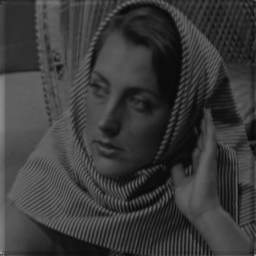
\includegraphics[width = \linewidth]{dct2D/barbara256 reconstructed using compressive measurements, without noise.png}
        \caption{Noiseless, 0.54114}
    \end{subfigure}
    \begin{subfigure}{0.24\linewidth}
        \centering
        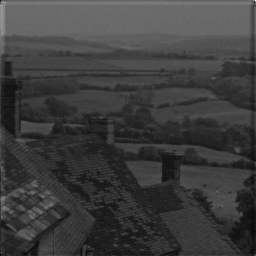
\includegraphics[width = \linewidth]{dct2D/goldhill reconstructed using compressive measurements, with noise.png}
        \caption{Noisy, 0.5414}
    \end{subfigure}
    \begin{subfigure}{0.24\linewidth}
        \centering
        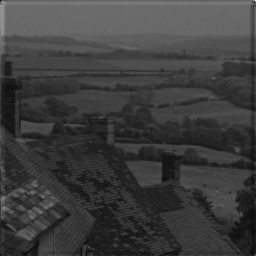
\includegraphics[width = \linewidth]{dct2D/goldhill reconstructed using compressive measurements, without noise.png}
        \caption{Noiseless, 0.5414}
    \end{subfigure}
    \caption{DCT Basis}
    \label{fig:dctb}
\end{figure}
\begin{figure}[H]
    \centering
    \begin{subfigure}{0.24\linewidth}
        \centering
        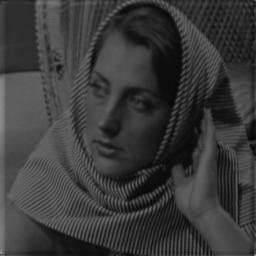
\includegraphics[width = \linewidth]{haarWavelet/barbara256 reconstructed using compressive measurements, with noise.png}
        \caption{Noisy, 0.54183}
    \end{subfigure}
    \begin{subfigure}{0.24\linewidth}
        \centering
        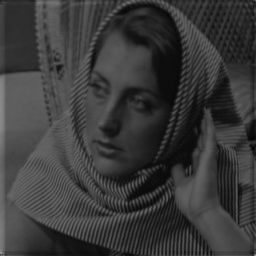
\includegraphics[width = \linewidth]{haarWavelet/barbara256 reconstructed using compressive measurements, without noise.png}
        \caption{Noiseless, 0.54184}
    \end{subfigure}
    \begin{subfigure}{0.24\linewidth}
        \centering
        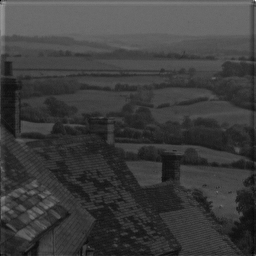
\includegraphics[width = \linewidth]{haarWavelet/goldhill reconstructed using compressive measurements, with noise.png}
        \caption{Noisy, 0.54209}
    \end{subfigure}
    \begin{subfigure}{0.24\linewidth}
        \centering
        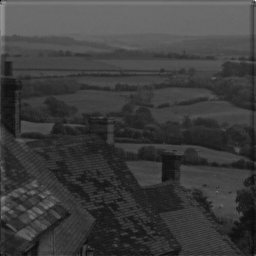
\includegraphics[width = \linewidth]{haarWavelet/goldhill reconstructed using compressive measurements, without noise.png}
        \caption{Noiseless, 0.54209}
    \end{subfigure}
    \caption{Haar Wavelet Basis}
    \label{fig:hwb}
\end{figure}
\end{document}